\newtheorem{definition}{定义}[section]
\newtheorem{example}{例}[section]
\chapter{背景知识}
为深入研究积木世界VQA中的空间推理问题,理解和掌握相关基础技术至关重要。本章将围绕本研究所依赖的核心技术
和数据集进行介绍,旨在为后续正式开展研究提供理论支撑与技术基础。
首先介绍 CLEVR 数据集,它是空间推理领域的经典数据集,
具有明确的物体属性、空间关系标签和程序化生成机制,其设计理念与积木世界高度契合,
是构建符合本研究的部分可见VQA数据集的重要参考依据。
其次,介绍回答集编程(Answer Set Programming, ASP),
它是一种基于非单调逻辑的知识表示与推理方法,具备高度表达能力和高效求解性能,
广泛应用于神经符号系统。
接着,介绍视觉语言预训练模型 GLIP,它能够实现图文联合理解和目标定位,为视觉信息的结构化提供强有力支持。
随后,将介绍近年来发展迅速的大语言模型(Large Language Models, LLMs),
特别是在规则生成与补全任务中的应用价值。
最后,介绍 DSPy 框架,目前其作为一种以程序化方式组织和优化大语言模型行为的开发工具得到了广泛应用。
\section{CLEVR数据集}
CLEVR(Compositional Language and Elementary Visual Reasoning)数据集是由 Johnson 等人于 2017 年
提出的一个用于评估视觉问答模型综合推理能力的合成数据集\cite{johnson2017clevr},
其设计初衷在于提供一个结构清晰、控制变量明确、便于自动标注的实验环境,
以有效分析VQA系统在多步推理、空间关系理解、属性比较与条件组合等方面的能力。
CLEVR 中的图像由多个具有不同几何形状、颜色、大小和材质的三维物体构成,生成方式基于程序控制的场景构建器,
从而保证了图像的可解释性与数据标签的完备性。问题与答案对则通过模板化方法自动生成,
每个问题背后对应一段形式化的程序,用于精确刻画其推理路径与中间步骤。

从视觉场景的构造逻辑来看,CLEVR 的设计理念与传统人工智能研究中的“积木世界”(\-Blocks World)高度一致,
二者均基于三维空间中多个物体的组合关系,并围绕空间布局、属性识别与对象间关系开展推理任务。
在 CLEVR 中,诸如“球体位于立方体的左侧”“红色物体后面有一个金属物体”这类问题与积木世界中的经典空间关系判断任务
在本质上具有相同的语义结构,因此,CLEVR 可被视为积木世界的一种程序化扩展与抽象建模,
其在空间推理表达的广度和精度方面提供了良好的基础支撑。由于其合成属性的可控性与逻辑严谨性,
CLEVR 被广泛用于神经符号推理模型的验证实验,成为空间推理型 VQA 任务的基准数据集之一。

然而,CLEVR数据集存在一些局限,具体表现在以下三方面:
\begin{enumerate}[nosep]
\item CLEVR中的场景完全可见。CLEVR数据集的图像中的场景都是完整的,即该图像对应的问题的全部所需信息均可从图像中获得,不需要其它外部的额外知识,
进而模型无需执行涉及隐藏信息的推理。场景完全可见的样例见图\ref{observable},其对应的自然语言问题是:“What color is the cube to the right of the small red metal cube?”。
由于该问题所涉及的所有物体在图\ref{observable}中完全可见,并且所有物体的各项属性(颜色、形状、大小、材质)非常清晰。
此外,问题中涉及的参照对象(小红色金属立方体)和目标对象(其右边的立方体)都在图中可以明确识别。
然而,在现实生活中部分可见性处处可见,例如扫地机器人在执行任务过程中的视角极其有限,
可能当前视野的图像中缺少判断前方是否存在障碍物的信息,此时需要一些关于该场景的额外知识,例如障碍物的图形学特征
等常识,辅助进行推理。
\begin{figure}[h]
    \centering
    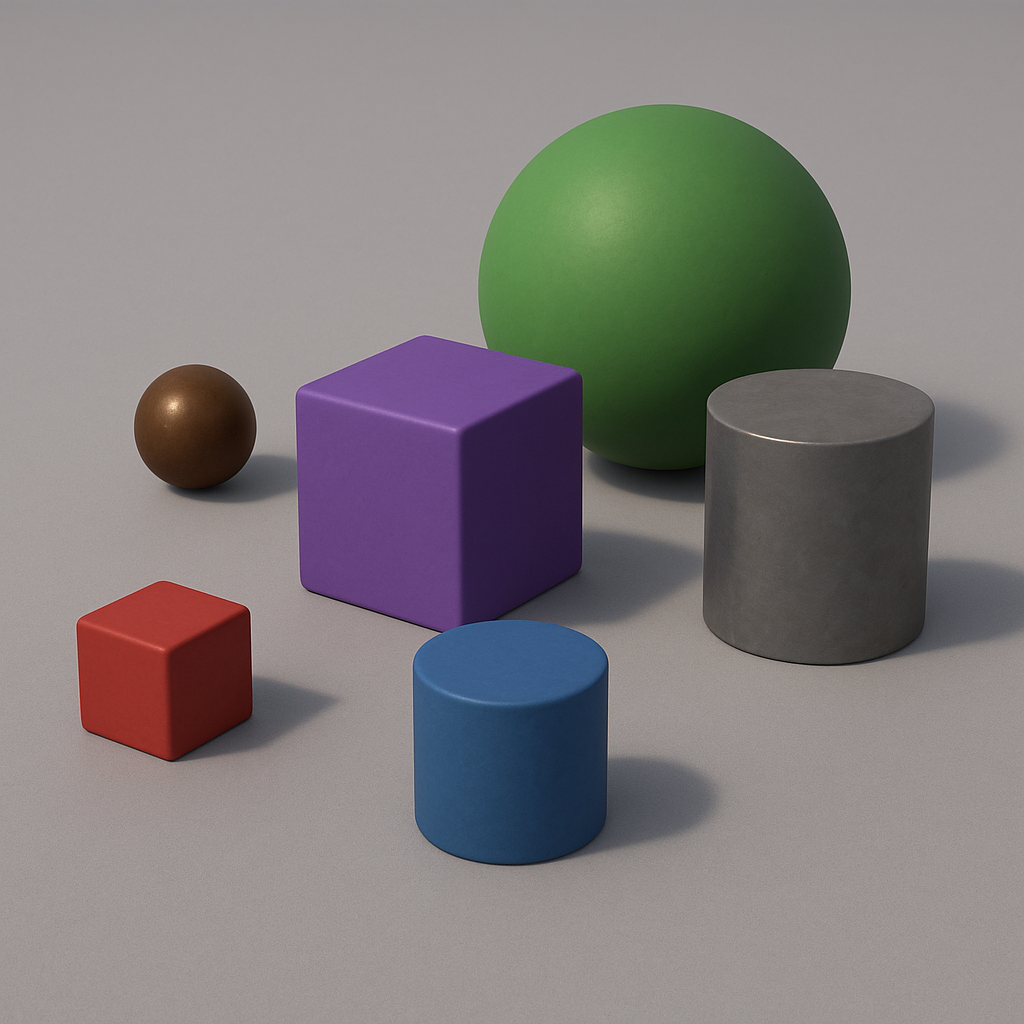
\includegraphics[scale=0.2]{figures/observable.png}
    \caption{CLEVR数据集中场景完全可见的样例}
    \label{observable}
\end{figure}
\item CLEVR缺乏显式表达背景知识或先验约束的机制。尽管CLEVR数据集旨在测试组合推理能力和基本视觉推理能力,
但其仅提供图像及图像中的对象属性,并不要求模型在回答问题时使用当前场景之外的、与当前场景相关的背景知识或逻辑约束。
在模型对CLEVR中的问题进行推理的过程中,模型主要依据对图像的直接理解和内部逻辑进行推理。仍以图\ref{observable}为例,
由于所有信息完全可见,故在该问题的推理过程中,模型不需要猜测、补全或者使用外部知识,
显然,真正的人工智能应该能够模仿人类的思考过程,根据问题所处的场景,灵活选取已有的相关知识,结合图像场景
的约束和问题的要求,进行推理。
% \item CLEVR中所有问题通常设计为唯一答案,未考虑部分可见场景这种不确定性条件之下的多解性问题。
% 在部分可见场景中,由于不确定性的存在,可能会有多个满足条件的物体或关系,导致问题的答案不唯一。
\end{enumerate}
以上两点局限导致模型在CLEVR数据集上获得的推理性能难以泛化至更具挑战性的实际应用场景,
尤其是在积木世界这类典型结构化环境中,部分可见性对问题求解结果具有显著影响。因此,
尽管 CLEVR 为空间推理的研究奠定了坚实基础,但仍需进一步构建具有部分可见性的VQA数据集,
以更真实地模拟积木世界中存在的不完全视觉信息问题。
\section{回答集编程}
% \numberwithin{equation}{section}
\subsection{语法}
项(terms)是ASP程序中最基本的元素,项可以是常量、变量或者函数。常量以符号常量或者数字表示(如4、a)。变量以字符串来表示,
要求首字母必须大写(如Dog、Person)。函数由函数符号与若干参数构成,例如$f(t_1,...,t_n),(n \geq 0)$。各参数
$t_i,(i=1,2,...,n)$也是项。若项中不存在函数符号与变量,则称该项为实例化项,否则称该项为非实例化项。

原子(atom)由谓词和项共同组成,例如$q(t_1,...,t_n),n \geq 0$。其中,$q$为$n$元谓词的标识符,$t_1,...,t_n$为项,
$n$为0时,谓词之后的括号可以省略。原子用于表示不同项之间的关系,例如:$dog(animal)$、$family(jensen,lucy)$、
$tomorrow\_sunny$,分别表示狗是动物、jensen和lucy是家人以及明天晴天。如果原子中的每一项都是实例化的,则该原子是实例化
原子,否则,该原子是非实例化的原子。例如,$dog(animal)$是实例化原子,$family(jensen,lucy)$是非实例化原子。
原子$q(t_1,...,t_n)$的强否定形式为$\urcorner q(t_1,...,t_)n$,其中符号$\urcorner$是经典逻辑中的否定,
$\urcorner q(t_1,...,t_n)$表示各项$t_i(1 \leq i \leq n)$。不符合
$q$所描述的关系,$\urcorner \urcorner a = a$,与经典逻辑中的排中律相同。文字(literal)可以是原子
$q(t_1,...,t_n)$,也可以是原子的强否定形式$\urcorner q(t_1,...,t_n)$。若文字对应的原子是实例化的,则称
该文字是实例化的。

\begin{definition}[规则] 规则$r$是具有如下形式的式子:
    \begin{equation}
        l_0 \thinspace or ... \thinspace or \thinspace l_m \leftarrow l_{m+1},...,l_n \thinspace not \thinspace l_{n+1},...,\thinspace not \thinspace l_p.
    \end{equation}
\end{definition}

其中$p \ge n \ge m \geq 0, l_i$代表文字,$not$为新的逻辑连接符,通常称作缺省否定符(default negation)或者
失败即否定(Negation As Failure, NAF),又称为若否定,$not \thinspace l_i$被读作“没有理由相信$l_i$为真”,但是这并不表明
$l_i$为假。对ASP程序而言,$not not a$不与a等价。规则r读作“如果相信$l_{m+1},...,l_n$为真,并且没有理由相信
$l_{m+1},...,l_p$为真,则相信$l_0 \thinspace or \thinspace ... \thinspace l_m$为真”。将$not l_i$称为缺省
文字(default literal),文字与缺省文字共同组成拓展文字(extended literal)。

规则$r$左侧的文字称为头部,可以表示为$head(r) = \{ l_0,...,l_m \}$。规则$r$右侧的文字称为体部,可以表示为
$body(r) = \{ l_{m+1},...l_n,not \thinspace l_{n+1},..., not \thinspace l_p \}$,规则的体部可以分为正
体部与负体部,正体部表示为$body^+(r) = \{ l_{m+1},...,l_n \}$,负体部表示为$body^-(r)=\{ l_{n+1},...,l_p \}$
。因此,规则$r$可以表示为:
\begin{equation}
    head(r) \thinspace \leftarrow \thinspace body^+(r), \thinspace not body^-(r) \label{con:body}
\end{equation}
一个ASP程序是有限条\eqref{con:body}所示的规则组成的集合。根据规则各部分所满足的相关条
件,可以分别定义事实、约束、正规规则、缺省规则和严格规则,如定义\eqref{def:fact}-定义\eqref{def:definite_rule}所
示。

\begin{definition}[事实]
当规则$r$满足$head(r)\neq \emptyset, body(r) = \emptyset$时,被称为事实(fact)。\label{def:fact}
\end{definition}
\begin{definition}[约束]
当规则$r$满足$head(r)= \emptyset, body(r) \neq \emptyset$时,被称为约束(constraint)。
\end{definition}
\begin{definition}[正则规则]
    当规则$r$满足$|head(r)|=1$时,被称为正则规则(normal rule)。
\end{definition}
\begin{definition}[缺省规则]
    当规则$r$满足$body(r)^-\neq \emptyset$时,被称为缺省规则(default rule)。
\end{definition}
\begin{definition}[严格规则]
    当规则$r$满足$body(r)^- = \emptyset$时,被称为严格规则(definite rule)。\label{def:definite_rule}
\end{definition}
根据上述各类规则的定义,本文进一步定义简单逻辑程序、缺省逻辑程序和正规逻辑程序如下。
\begin{definition}[简单逻辑程序]
    若程序$P$由有限条严格规则组成,则$P$被称为简单逻辑程序。
\end{definition}
\begin{definition}[拓展逻辑程序]
    若程序$P$由有限条缺省规则组成,则$P$被称为拓展逻辑程序。
\end{definition}
\begin{definition}[正则逻辑程序]
    若程序$P$除约束外,由有限条正则规则组成,则$P$被称为正则逻辑程序(Normal Logic Program, NLP)。
\end{definition}
若不做特别说明,本文考虑的程序均为不含约束的正规逻辑程序,即程序中的每条规则头部有且仅有一个文字。
\subsection{语义}
\subsubsection{文字的可满足性语义解释和程序的模型}
作为基础理论,首先给出 Herbrand 域、Herbrand 基的定义,分别如定义2.10和2.11所
示,进一步定义规则与程序的实例化,最终在实例化程序下讨论文字的可满足性语义解
释和可满足性。
\begin{definition}[Herbrand基]
    $P$是一个 ASP 程序,将程序$P$中出现的常量和函数形成的
    所有不含变量的项的集合称为 Herbrand 域,使用$\mathcal{U}_P$表示。
\end{definition}
\begin{definition}[Herbrand域]
    $P$是一个 ASP 程序,出现在程序$P$的规则中的谓词符号与
$\mathcal{U}_P$中的项组成的所有可能的不含变量的原子集合称为程序$P$的 Herbrand 基,使用$\mathcal{A}_P$
表示,为了保持简洁,通常简写为$\mathcal{A}$。
\end{definition}
\begin{definition}[规则的实例化]
    给定$P$中的一个规则$r$,使用$ground(r)$表示通过使用
$\mathcal{A}_P$中的常量对应地替换$r$中变量而获得的规则集合,这一映射被称为规则的实例化。
\end{definition}
\begin{definition}[程序的实例化]
    程序$P$由一系列规则的集合组成,程序$P$的实例化$ground(P)$表示为式\eqref{equation:ground}:
    \begin{equation}
    ground(P)=\bigcup_{r \in P}ground(r) \label{equation:ground}
    \end{equation}
\end{definition}
\begin{definition}[文字的可满足性语义解释]
    定义文字的可满足性语义解释$I=\langle I^+,I^- \rangle$,其中$I^+\cup I^-\subseteq \mathcal{A}_P$
    ($P$是实例化程序),$I^+\cap I^-=\emptyset$。$I^+$表示为已知为真的文字集合,$I^-$表示已知为假
    的文字集合。当$I^+\cap I^-=\mathcal{A}_P$时,$I$被称作完全可满足性语义解释(complete interpretation)。
    若I不是完全可满足性语义解释,则$I$中存在真值未确定(undefined)的文字。
\end{definition}
\begin{definition}[程序的模型]
    假设$P$是一个实例化的回答集程序,$I=\langle I^+,I^- \rangle$是一个可满足性语义解释。若文字$l \in I^+$,
    则称I满足$l$,记作$I\models l$;对缺省文字$not l$,若$l \in I^-$,则称I满足$not l$,记作$I\models not l$。
    对于文字集合$S$,若$\veebar l \in S,I \models l$,则称$I$满足集合$S$,记作$I \models S$,当一个规则
    $r$满足$I \nvDash body(r)$或$I \models head(r)$时,$I$满足规则$r$。当$I$满足程序$P$的所有规则时,称
    $I$是$P$的一个模型。
\end{definition}
\subsubsection{回答集语义}
\begin{definition}[一致性文字集合]
    给定一个文字集合$S$,若$S$中不同时包含$l$和$\urcorner l$,则集合S是一致性文字集合,其中,$l \in S$是集合
    S中的任意文字。
\end{definition}
\begin{definition}[可满足性,Satisfiability]
    给定一致性文字集合$S$,文字$lit$与规则 $r$,若
$lit \in S$,则文字$ lit $满足集合 $S$。若 $head(r)\cap S \neq \emptyset$,则 $S $满足头部。若$ body^+(r) \subseteq 
S, S ∩ body^−(r) = \emptyset$,则集合$ S $满足体部。若 $S $满足规则 $r$ 的头部或者 $S $不满足规则$ r$ 的
体部,则$ S$满足规则 $r$,记作$ S \models r$。给定一个 ASP 程序 $P$,若 $\veebar r \in P, S \models r$,则 $S$ 满足
程序 $P$。
\end{definition}
\begin{definition}[规则的适用与阻塞]
    给定一致性文字集合 $S$ 与规则 $r$,$S$ 满足 $body(r)$,
则称规则 $r $在集合$S $下是适用的(applicable),否则称规则$ r $在集合$ S$ 下被阻塞(block)。
\end{definition}
\begin{example}
    给定ASP程序$P_3$,该程序包含两条规则:
    \begin{align*}
        &r_1: p \leftarrow q, s. \\ 
        &r_2: s \leftarrow t.
    \end{align*}
\end{example}
下面通过分析说明集合$S=\{ p, q\}$对程序$P$的可满足性。
\begin{enumerate}[nosep]
    \item 因为$p\in S$,所以文字$p$与文字$q$均满足$S$;
    \item 因为$S \cap head(r_1) = \{ p \} \neq \emptyset$,所以$S$满足$head(r_1), S \models r_1$;
    \item 因为$body^+(r_2) \subsetneq S$,所以$S$不满足$body(r_2)$,所以$S \models r_2$;
    \item 因为$S$满足程序$P$中的每一条规则,所以$S$满足程序$P$。
\end{enumerate}
\begin{definition}[Gelfond-Lifshitz规则(GL规约)]
    假设程序 $P$ 是给定的实例化程序,$S$
是一致性文字集合,$l$ 是文字,$S \subseteq  Lit(P), l \in Lit(P)$, $P $关于 $S$ 的$ GL$ 规约结果$ P^S$定义为式\eqref{equation:GL}:
\begin{equation}
    P^S = \{ head(r) \leftarrow body^+(r) \mid r \in P, body^-(r) \cap S = \emptyset \} \label{equation:GL}
\end{equation}
\end{definition}
\begin{definition}[简单逻辑程序回答集\cite{}]
    假设$P$是简单逻辑程序,程序$P$的回答集是$S \subseteq Lit(P)$ 满足:

    \begin{enumerate}[nosep]
        \item 对于程序$P$中的每一条规则$l_0 \leftarrow l_1,...,l_m$,如果$l_1,...,l_m \in S$,那么$l_0 \in S$。
        \item $S \subseteq Lit(P)$且不存在$ S$ 的任何子集也满足程序 $P$ 的每一个规则,即 $S $是满足程序$ P$的最小集合;
        \item 如果 $S$ 包含互补的文字,那么 $S = Lit(P)$;
    \end{enumerate}
\end{definition}
\begin{definition}[拓展逻辑程序回答集]
    假设$P$是包含缺省否定的扩展逻辑程序,$S$是实例化文字集合,如果$S$是$P^S$的回答集,则$S$是$P$的回答集。如果程序$P$没有回答集或
者只有一个包含互补文字的回答集$Lit(P)$,那么程序$P$是不一致程序,否则,程序$P$是一致性程序。

可以看出,使用 GL 规约,可以将扩展逻辑程序程序转换为简单逻辑程序,从而得到扩展逻辑程序的回答集。下面通过一个例子说明。
\begin{example}[GL规约与问答集]
    给定一个实例化的ASP程序$P_4$:
    \begin{align*}
        &r_1: p(a) \leftarrow not p(b) \\
        &r_2: p(b) \leftarrow not p(a) \\
        &r_3: \leftarrow p(b).
    \end{align*}
    程序$P_4$可能的回答集有四个:$S_1 = \emptyset, S_2 = \{ p(a) \}, S_3 = \{ p(b) \}, S_4 = 
    \{ p(a), p(b) \}$, 根据回答集的定义依次验证:
    \begin{enumerate}[nosep]
        \item $P^{S_1} = \{ p(a) \leftarrow .\} \cup \{ p(b) \leftarrow . \} \cup \{ \leftarrow p(b) .\}$,事实$(p(b) \leftarrow .)$
    与约束$(\leftarrow p(b).)$同时在$P^{S_1}$中出现,因此$S_1$不是$P^{S_1}$的回答集,所以$S_1$不是$P$的回答集。
        \item $P^{S_2} = \{ p(a) \leftarrow .\} \cup \{ \leftarrow p(b) .\}$,而$S_2 \models ((p(a) \leftarrow .))$且
    $S_2 \models (\leftarrow p(b).)$,因此$S_2 \models P^{S_2}$,且不存在$S_2^{'}\subset S_2, S_2^{'} \models P^{S_2}$,所以$S_2$是$P^{S_2}$的回答集;

        \item $P^{S_3} = \{ p(b) \leftarrow . \} \cup \{ \leftarrow p(b) .\}$,事实$(p(b) \leftarrow .)$
    与约束$(\leftarrow p(b).)$同时在$P^{S_3}$中出现,因此$S_3$不是$P^{S_3}$的回答集,所以$S_3$不是$P$的回答集;
        \item $P^{S_4} = \{ \leftarrow p(b). \}$,可知$P^{S_4}$的回答集为$\emptyset$,因此$S_4$不是
    $P^{S_4}$的回答集,所以$S_4$不是$P$的回答集。
    \end{enumerate}
\end{example}
\end{definition}

\subsubsection{well-founded语义}
上世纪 90 年代,良基语义(well-founded semantics)的概念由 Van Gelder A 提出,
对于任意的回答集程序,都存在对应的良基模型(well-founded models),并且在多项式
时间内可以计算出这个模型\cite{van1991well}。该语义模型是本文对 NAF 文字进行解释和对不一致程
序原因进行分类的重要基础,下面介绍这一模型的定义及计算方法。

\begin{definition}[立即结论]
$P$是一个 ASP 程序,$S\subseteq \mathcal{A}_P,V\subseteq \mathcal{A}_P$,则集合$S$关于$P$和$V$的
立即结论(immediate consequence)记作 $\mathcal{T}_{P,V}(S)$,定义如式\eqref{equation:immediate_consequence}所示:
\begin{equation}
    T_{P,V}(S) = \{ a | \exists r \in P, head(r) = a, body^+(r) \subseteq S, body^-(r)\cap V = \emptyset \} \label{equation:immediate_consequence}
\end{equation}
\end{definition}
考察上式可以发现,当集合$V$确定时,关于集合$S$的函数$T_{P,V}(S)$是单调的。因此,当集合$V$固定时,该函数
存在最小不动点(Least Fixed Point, LFP),使用$lfp(.)$表示。

\begin{definition}[良基模型]
    $P$是一个 ASP 程序,$P^+$是程序$P$中的全部严格规则的集合,序列$(K_i,U_i)_{i \geq 0}$定义如下:
    \begin{align*}
        &K_0 = \mathit{lfp}(T_{P^+}) & K_i &= \mathit{lfp}(T_P, U_{i-1}) \\
        &U_0 = \mathit{lfp}(T_{P, K_0}) & U_i &= \mathit{lfp}(T_{P, K_i})
    \end{align*}
\end{definition}
若$\langle K_j,U_j \rangle = \langle K_{j+1},U_{j+1} \rangle$,且不存在$0 \leq k < j$,使得
$\langle K_k, U_k = \langle K_{k+1},U_{k+1} \rangle$(j,k是正整数),则$P$的良基模型$WF_P=\langle W^+,W^- \rangle$,
满足$W^+=K_j$,$W^-=\mathcal{A}\backslash U_j$
\begin{example}[良基模型]
    程序$P_5$包含以下四条规则:
    \begin{align*}
        &r_1:q \leftarrow , not p. &r_2: p \leftarrow, not q. \\
        &r_3:a \leftarrow b. &r_4: b \leftarrow. 
    \end{align*}
\end{example}
首先得到$P_5^+=\{ a \leftarrow b \} \cup \{b \leftarrow . \}$,而$lfp(T_{P_5^+}) = {a, b}$,因此
$K_0 = {a,b}$;进一步计算得到$U_0 = lfp(T_{P_5^+, K_0}) = \{ a,b,p,q \}$,$K_1 = lfp(T_{P_5^+, U_0}) = 
\{ a, b \} = K_0$,$U_1 = lfp(T_{P_5^+,K_1}) = \{ a,b,p,q \} = U_0$。因此$\langle K_0, U_0 \rangle = 
\langle K_1, U_1 \rangle$且不存在$0 \leq k < 1$,$\langle K_k, U_k \rangle = \langle K_{k+1}, U_{k+1} \rangle$。
因此程序$P_5^+$的良基模型为$WF_{P_5^+} = \langle \{a, b\}, \{ \} \rangle$,$p$和$q$在良基模型中属于
未定义($undefined$)。
\subsection{ASP求解器}
ASP求解器是实现ASP语义推理的核心工具,其工作原理是:通过搜索逻辑程序的最小模型(即回答集)来解决复杂的组合优化问题。

ASP求解器的工作流程可以划分为两个阶段:基础化(Grounding)和求解(Solving)。
基础化是将一阶逻辑程序实例化为命题逻辑形式,而求解则是基于CDCL算法搜索满足约束的模型。

截至目前,已经有众多ASP求解器。学术界和工业界所用的主流的求解器,可分为两类:单阶段求解器(如Clasp、DLV)、
多阶段求解器(如Clingo)。两类求解器的主要区别在于,单阶段求解器独立地进行基础化与求解,而多阶段求解器
则是集成了基础化与求解的交互式系统。

表\ref{tab:solver_comparison}对目前的主流ASP求解器的适用场景及核心优势进行了对比。因为 Clingo 求解器
具有免费开源、使用简单、运行高效的特点,本文在求解 ASP程序时,使用 Clingo 进行相关实验。
\begin{table}[h]
    \centering
    \renewcommand{\arraystretch}{1.2}
    \begin{tabular}{l l l l}
        \toprule
        \textbf{求解器} & \textbf{核心技术} & \textbf{适用场景} & \textbf{核心优势} \\
        \midrule
        \multirow{2}{*}{Clasp} & 多线程CDCL & 大规模组合优化 & 支持并行搜索 \\
                               & 情性子句学习 & 工业级应用 & 性能竞赛冠军 \\
        \midrule
        \multirow{2}{*}{Clingo} & 增量式基础化 & 动态规则生成 & 集成Python API \\
                                & 多阶段编程 & 交互式推理 & 支持在线更新程序 \\
        \midrule
        \multirow{2}{*}{DLV} & 数据库优化 & 知识表示型问题 & 高效处理复杂规则 \\
                             & 存在线量化推理 & 语义Web & 支持非确定域 \\
        \midrule
        \multirow{2}{*}{WASP} & 分层弱约束优化 & 偏好推理 & 加权约束高效处理 \\
                              & 冲突驱动剪枝技术 & 多目标优化 & \\
        \midrule
        \multirow{2}{*}{Smodels} & 稳定模型算法 & 教学与研究 & 算法透明易扩展 \\
                                 & 部分求值 & 基础模型验证 & \\
        \midrule
        LPARSE & 基础化预处理 & 规则实例优化 & 与Smodels配合使用 \\
        \midrule
        \multirow{2}{*}{IDP} & 基于模型的推理 & 复杂知识库管理 & 支持类型系统 \\
                             & 扩展一阶逻辑 & & 高阶推理 \\
        \midrule
        Alpha & 并行求解引擎 & 超大规模问题 & GPU加速搜索 \\
        \bottomrule
    \end{tabular}
    \caption{扩展后的系统对比}
    \label{tab:solver_comparison}
\end{table}
\section{GLIP}
在积木世界VQA任务中,系统需要准确识别图像中的各类几何体、理解其属性(如颜色、材质、形状)、
定位其空间位置,并将这些视觉事实转化为结构化的符号信息,供符号推理模块进行逻辑推演。
因此,目标检测模块不仅需要具备高精度的检测能力,还应能支持丰富灵活的语言描述,以适应多样化的问答形式。
在本研究构建的神经符号VQA框架中,GLIP(Grounded Language-Image Pretraining)被选为核心的视觉解析组件,
其通用性与语言驱动检测能力为后续的视觉场景理解提供了关键支持。

GLIP 是一种基于图文对齐预训练的目标检测框架,旨在统一视觉识别与自然语言理解任务。
与传统检测模型如 Faster R-CNN、YOLO 系列或 DETR 不同,这些模型依赖于封闭类别集合进行训练和推理,
难以适配于用户自定义或开放式的语言查询。而 GLIP 的创新点在于引入 语言提示(language prompts) 
作为查询机制,允许用户以任意自然语言短语描述待检测目标,
从而实现开放词汇(open-vocabulary)目标检测\cite{li2022grounded}。
GLIP 的这一特性尤为适合积木世界VQA场景中涉及“最右边的紫色圆柱体”“靠近红球体的黄色立方体”等组合性语言
表达的识别需求。

GLIP的架构如图\ref{GLIP_architecture}所示,从架构上看,GLIP 借鉴了 DETR 的端到端检测思想,整体由以下几个模块构成:
\begin{enumerate}[nosep]
\item 视觉编码器:通常为ViT(Vision Transformer)或ResNet,将图像编码为空间维度保留的特征张量;
\item 文本编码器:采用 BERT 或类似的 Transformer 模型,将输入语言提示转换为语义嵌入;
\item 跨模态交互模块:引入 Cross-Attention 机制,实现图文特征的融合对齐;
\item 检测头(Detection Head):利用融合后的特征对每个语言提示生成目标框位置与匹配分数。
\end{enumerate}
\begin{figure}[h]
    \centering
    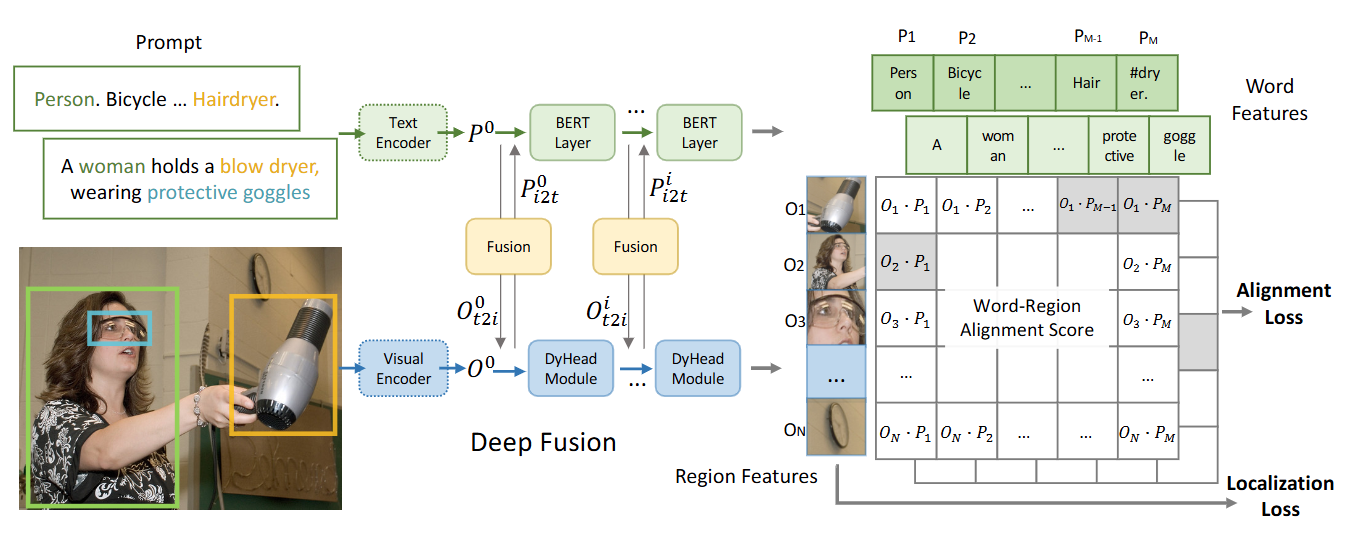
\includegraphics[width=\textwidth]{GLIP_architecture.jpg}
    \caption{GLIP结构示意图\label{GLIP_architecture}}
\end{figure}

该模型在训练阶段采用了包含图像-文本对的大规模预训练语料(例如 Visual Genome 和 Objects365 等),
使得其具备强大的跨模态语义匹配能力。实验结果表明,GLIP 在开放词汇目标检测任务中的平均精度(mAP)
显著优于传统检测框架,并在下游视觉问答、图文匹配等任务中展现出出色的迁移性能\cite{li2022grounded}。

在本研究中,GLIP 被用于将积木世界图像中的物体及其属性结构化为三元组形式,
如 object(sphere, red, leftmost),这些三元组作为输入供 ASP 推理
模块进行空间关系推理。与基于固定类标的目标检测方法相比,GLIP 的语言可控性显著降低了对类别词表的依赖,
使得系统具备更强的扩展性与灵活性,尤其适应于问答任务中动态变化的问题语境。

综上,GLIP 凭借其开放词汇检测能力、图文联合建模机制以及良好的通用性,
成为本研究神经符号VQA框架中的关键视觉组件。它不仅提升了积木世界图像结构化建模的准确性,
还显著增强了系统对复杂语言问句的适应能力,为构建高效、可解释的空间推理VQA系统提供了坚实基础。
\section{大语言模型}
在本文提出的神经符号VQA框架中,大语言模型(Large Language Models, LLMs)在多个关键模块中发挥了核心作用。
我们主要采用了 ChatGPT、LLaMA 和 DeepSeek 三种主流模型。
它们各自具备不同的特点和优势,以下将对这三种主流模型展开介绍。
\subsection{GPT}
目前,GPT系列最新的模型为GPT-4o,其在架构方面采用了高达1.8T参数的多模态Transformer,引入联合注意力机制,支持文本-图像-语音跨模态联合推理。
此外,GPT采用了动态窗口扩展技术,长文本生成连贯性指标提升37\%。

训练策略上,采用了强化学习对齐(RLHF)​,通过3阶段训练(SFT → RM → PPO),有害内容生成率降至0.3\%。
并且采用了​数据蒸馏的方案,其使用合成数据占比达45\%,有效减少了网络噪声数据污染。

GPT目前在​多模态理解方面表现优异,图像描述任务BLEU-4达0.74,视频内容摘要准确率91\%。
然而GPT训练成本高昂,价格较高,每百万token费用7.5美元,是DeepSeek的53倍。
\subsection{LLaMA}
LLaMA是由Meta开源的LLM,其在架构上采用​分组查询注意力(GQA),​键值头数量压缩至查询头的1/4,70B模型推理显存需求降至48GB。
此外,还采用了​RoPE位置编码,动态旋转嵌入技术提升长文本连贯性,32k上下文下困惑度降低12\%。

训练策略上,LLaMA​采用了课程学习策略,分阶段增加数据复杂度,代码生成任务准确率提升19\%。
此外,LLaMA还支持​量化部署,4bit量化版可在消费级显卡(RTX 4090)运行,大大降低了模型的部署应用门槛。

​LLaMA-3整合CLIP视觉编码器,使其在多模态领域具有较强的应用能力,图像问答VQA准确率82\%。
\subsection{DeepSeek}
在架构层面上,DeepSeek采用了混合专家架构(MoE)​、​多头潜在注意力(MLA)以及动态路由策略,以更好地对训练过程进行优化,降低
对硬件的需求。其采用细粒度专家分割(256个路由专家+1个共享专家),激活参数仅占全量参数的1/10,推理速度提升3倍。
此外,DeepSeek还通过低秩键值压缩技术,将KV缓存需求降低60\%,支持64k token长上下文处理(约3-4万字)。基于负载均衡优化算法,专家利用率提升30\%,在代码生成任务中HumanEval得分达53.8\%。

在训练优化上,DeepSeek使用了FP8混合精度训练的方案,结合BF16与FP8量化,单卡H800训练吞吐量提升2.1倍,175B模型训练成本降至OpenAI的1/10。
此外,也采用了​强化学习优先(RL-First)​的策略,DeepSeek-R1通过纯强化学习训练实现复杂推理,数学证明任务准确率比GPT-4o高15.4\%。

相比目前其它的LLM,DeepSeek对硬件的需求更小,应用场景拓展到了移动端本地部署。
此外,DeepSeek的高推理速度也使得其被应用于实时风险分析领域,某银行系统响应延迟压缩至200ms。
\subsection{LLM总结}
目前,LLM的产业化应用已渗透至许多行业,在金融、教育、法律等领域大显身手。

头部投行部署GPT-4o模型实现高频交易策略优化,实时解析财经新闻、财报电话会议录音,构建情感指数(Sentiment Index),预测标普500指数波动率的误差率仅2.3\%;
​通过强化学习动态调整投资组合,在2024年美股波动期间最大回撤控制在5\%以内,优于人工策略的12\%;
LLM自动解析《巴塞尔协议III》等法规文件,识别交易记录中的异常模式,某欧洲银行借此将反洗钱审查效率提升40倍。

在线教育平台“学而思”集成LLaMA-3模型开发智能辅导系统,根据学生答题数据(如错误知识点关联图)动态生成习题,某初中数学实验班平均成绩提升23\%;
采用多维度评估框架(逻辑性、语法、创新性),与教师评分的一致性系数(Cohen's Kappa)达0.81;
7×24小时解答学科问题,在江苏省高三模拟考中,系统对物理压轴题的解题正确率超过95\%。

某顶级律所联合DeepSeek-R1模型构建法律智能平台,扫描百万字合同文本,自动标记非常规条款(如对赌协议中的隐藏风险),准确率98.7\%;
基于历史案例数据库,对知识产权纠纷案的胜诉概率预测与法院判决吻合度达89\%;将法律意见书起草时间从40小时压缩至2小时,且符合《民法典》最新司法解释要求。

尽管LLM取得突破性进展,仍需解决以下问题。
\begin{enumerate}[nosep]
\item ​高质量语料短缺与数据多样性不足的问题。训练GPT-4和Gemini Ultra需要4-8万亿单词,而人类高质量文本数据可能在2026年前耗尽。中文语料尤其匮乏,全球大模型训练集中文占比仅1.3\%,且国内缺乏垂直领域专用数据集。此外,共享语料库存在大量噪声,例如社交媒体内容碎片化、标注不一致等问题,直接影响模型性能。例如,化工行业安全检查单需通过LLM重新筛选和优化低相关性条款。
\item 模型扩展定律(Scaling Laws)的失效。OpenAI新一代模型Orion在训练进度20\%时达到GPT-4水平,但后续投入更多资源后性能提升不足5\%,显示传统“堆参数”模式已遇瓶颈。此外,GPT-4单次推理成本达数万次浮点运算,日均调用百万次的企业算力成本超数万美元,而模型能力提升与成本增长不成正比。
\item 幻觉(Hallucination)与可靠性缺陷问题。LLM在缺乏数据支撑时可能编造虚假信息,例如谷歌Bard错误描述天文照片来源。金融、医疗领域因此面临业务风险,某法律分析系统需人工审核降低误判率。
\item 推理效率与速率限制。GPT-4推理需40GB显存,平均响应延迟超3秒,远超用户容忍阈值。异步函数调用技术(如AsyncLM)通过并行化处理,可将任务加速5.4倍,缓解了这一问题,但仍需硬件优化。
\end{enumerate}
\section{DSPy}
为了实现大语言模型与符号推理模块之间的高效协同,
近年来出现了一种新型编程范式——声明式语言模型编程(Declarative LLM Programming)。
DSPy(Declarative Self-improving Python)正是该范式的代表性框架。
它通过模块化、声明式的方式,将语言模型调用与复杂任务逻辑解耦,极大地简化了神经符号系统的构建流程。

DSPy 将语言模型视为可组合的模块(Modules),如 Prompt, ChainOfThought, ReAct, Retrieve, Select 等,
并支持在这些模块中嵌入目标任务的“意图说明”(specifications)。它最突出的特点包括:
\begin{enumerate}[nosep]
\item \textbf{声明式建模}:用户只需定义“输入-输出要求”,而不需要手动编写 Prompt 或控制模型细节。
\item \textbf{程序级优化}:框架通过训练、调优或样例注入自动优化模块表现,具备一定的自我改进(Self-improvement)能力。
\item \textbf{LLM-agnostic 架构}:DSPy 可无缝对接 ChatGPT、LLaMA、DeepSeek 等多种 LLM,提升了系统的灵活性与可移植性。
\end{enumerate}

DSPy 所具备的可组合性、可解释性和与 LLM 的深度集成能力,
使其成为构建“可控”“结构化”“可调试”的神经符号框架的理想桥梁。
与传统的 Prompt 工程相比,DSPy 更适合构建语义导向、规则驱动的VQA系统,
特别是在空间推理任务中,其对规则生成、语义一致性与模型泛化能力提供了有力支持。
\section{本章小结}
首先介绍 CLEVR 数据集,该数据集与积木世界高度契合,是构建符合本研究的部分可见VQA数据集的重要参考依据。
其次,介绍回答集编程(Answer Set Programming, ASP),围绕其语法、语义以及不同类型的ASP求解器展开了介绍。
接着,介绍本文所用的视觉语言预训练模型 GLIP,它能够实现图文联合理解和目标定位,为视觉信息的结构化提供强有力支持。
随后,将介绍近年来发展迅速的大语言模型(Large Language Models, LLMs),并对当前LLM发展需要解决的问题和LLM目前已经应用的领域展开介绍。
最后,介绍 DSPy 框架,其作为一种以程序化方式组织和优化大语言模型行为的开发工具,在本研究中被用于迭代反馈与规则修正环节的提示词学习。本章介绍的众多技术手段,为后续进一步开展研究提供了重要保障。